\section{Aplicação}

\begin{frame}{Aplicação}
	\begin{figure}[h]
		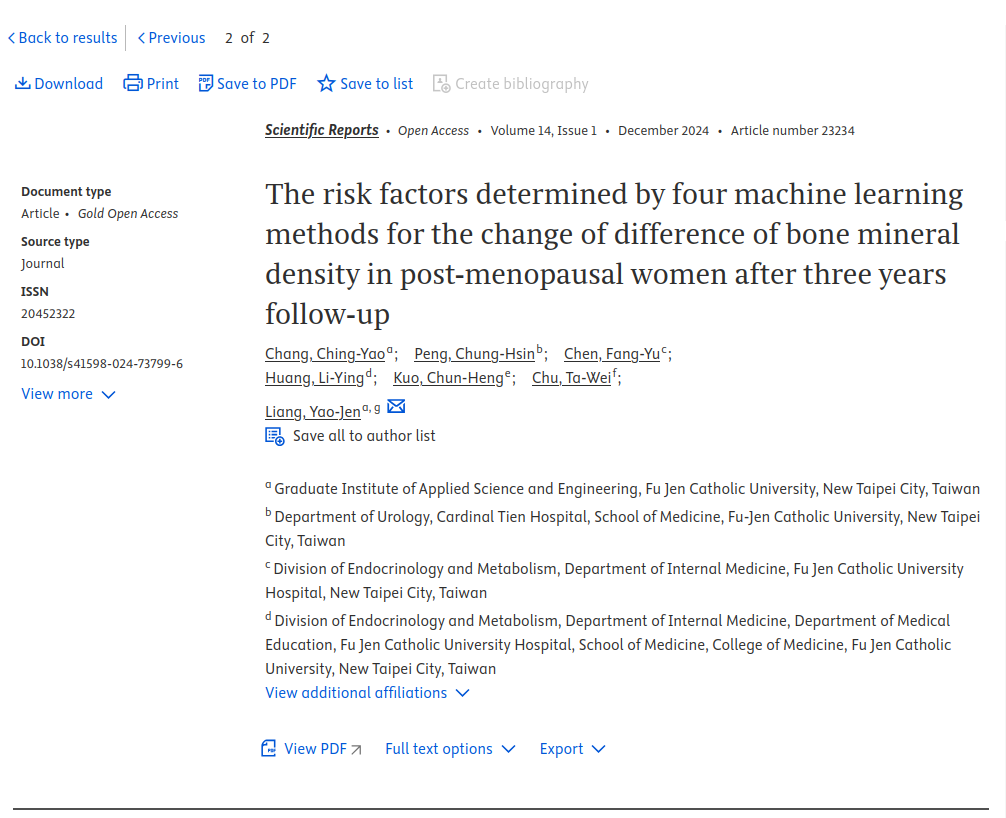
\includegraphics[scale=0.3]{imagens//secao3/artigo2.png}
	\end{figure}
\end{frame}

\begin{frame}{Contextualização}
	\begin{block}{Osteoporose}
		é uma doença em que a degradação estrutural e a diminuição da densidade mineral dos ossos (DMO) aumentam o risco de fraturas ósseas.
	\end{block}
	\pause
	\begin{block}{Motivações para o estudo}
		\begin{itemize}
			\item  A prevalência da osteoporose aumentou drasticamente nos últimos anos;
			\item  Representa um problema de saúde pública com alto índice de morbidade (muito comum).
		\end{itemize}
	\end{block}
\end{frame}

\begin{frame}{Contextualização}
	\begin{block}{}
		\begin{itemize}
			\item Em 2010, na União Europeia, aproximadamente 5,5 milhões de homens e 22 milhões de mulheres foram afetados pela osteoporose;
			\item 80\% das mulheres afetadas não estavam cientes dos seus fatores de risco até o diagnóstico.
		\end{itemize}
	\end{block}
\end{frame}

\begin{frame}{Objetivos}
	\begin{block}{}
			\begin{enumerate}
			\item Comparar a precisão preditiva dos métodos aprendizado de máquina com a regressão linear múltipla tradicional;
			\pause
			\item Classificar a importância de vários fatores de risco, incluindo dados demográficos, estilo de vida e bioquímica, na previsão das mudanças futuras no $\delta$-T score.
		\end{enumerate}
	\end{block}
\end{frame}

\begin{frame}{Fonte dos Dados}
	\begin{block}{}
		\begin{itemize}
			\item Coorte MJ de Taiwan  
			\item Exames conduzidos pelos Centros de Triagem de Saúde MJ  
		\end{itemize}
	\end{block}
\end{frame}

\begin{frame}{Informações Coletadas}
	\begin{itemize}
		\item Mais de 100 indicadores biológicos essenciais  
		\pause
		\item Questionário abrangendo: 
		\pause 
		\begin{itemize}
			\item Histórico médico pessoal e familiar  
			\item Estado de saúde atual  
			\item Estilo de vida e exercício físico  
			\item Hábitos de sono e alimentares  
		\end{itemize}
	\end{itemize}
\end{frame}

\begin{frame}{Considerações Éticas}
	\begin{itemize}
		\item Consentimento informado dos participantes  
		\item Aprovação pelo Comitê de Ética
	\end{itemize}
\end{frame}

\begin{frame}{Seleção da Amostra}
	\begin{figure}[h]
		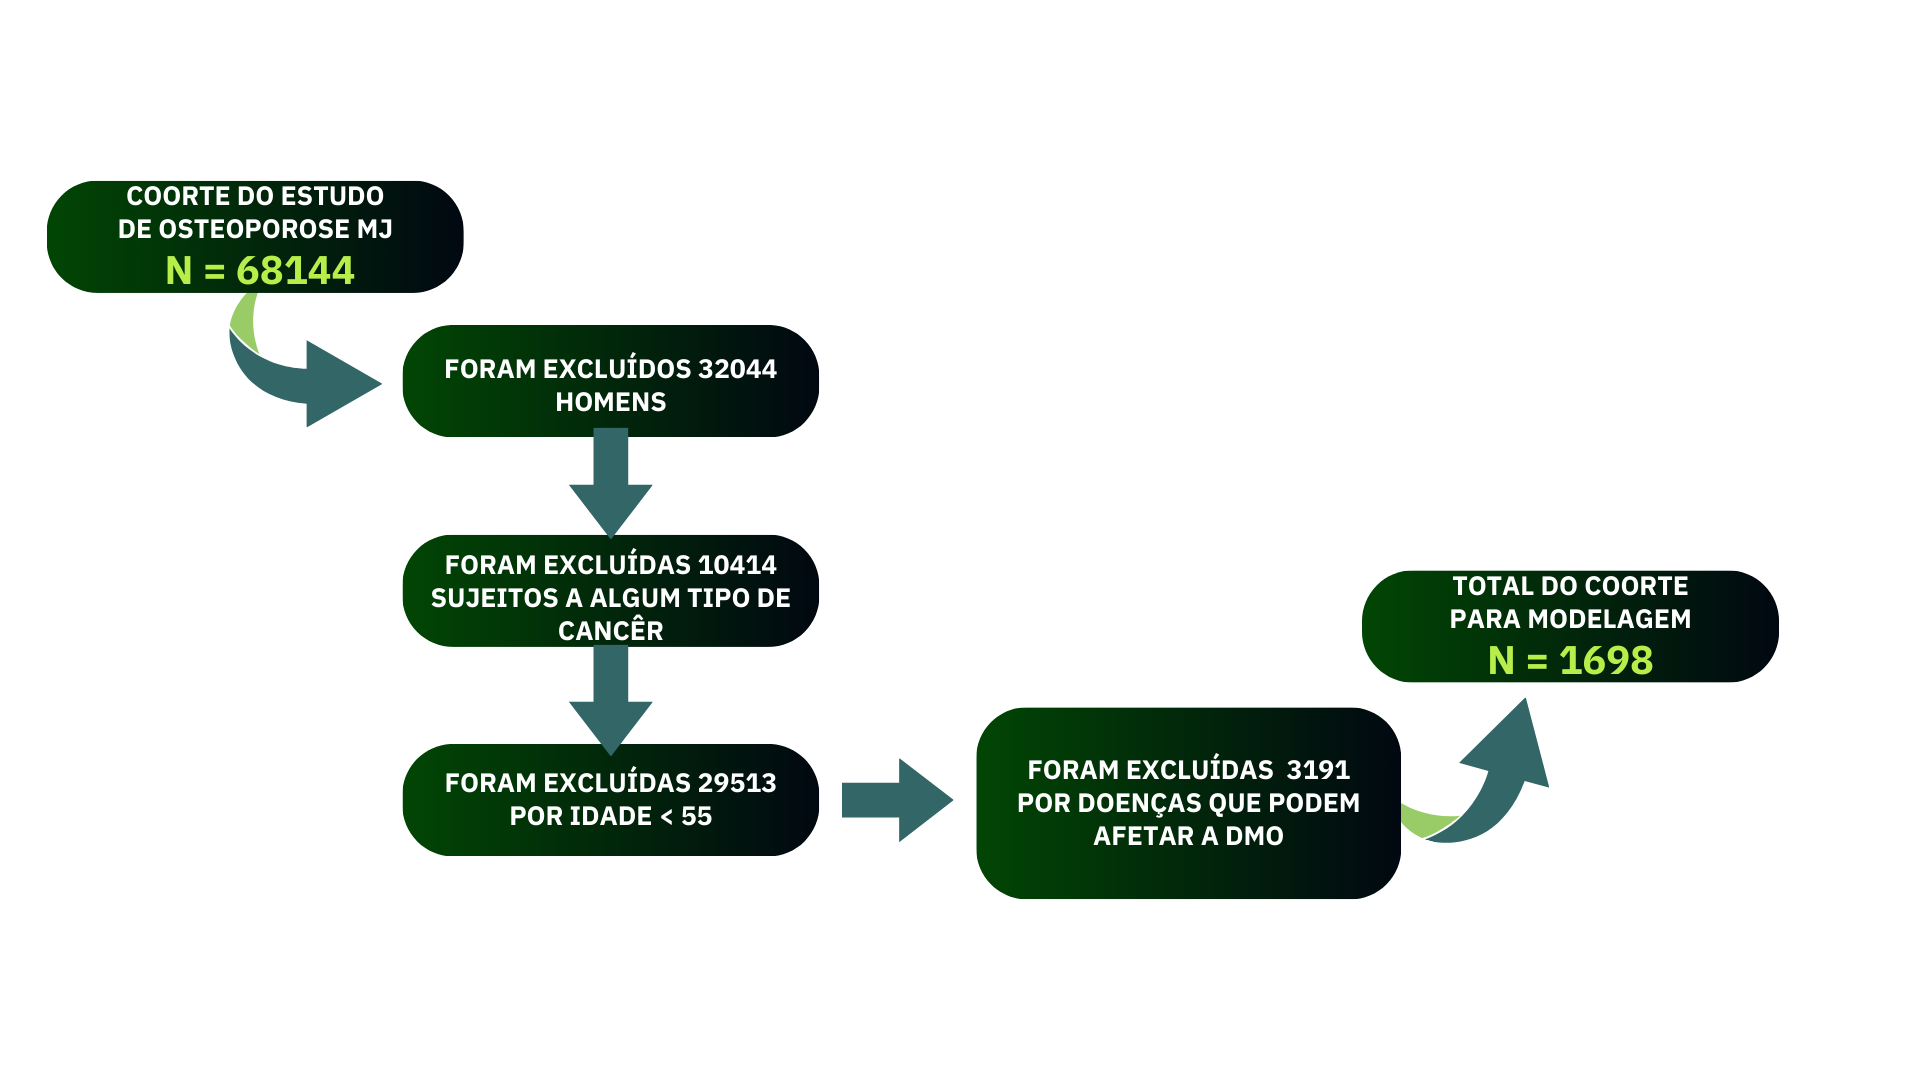
\includegraphics[width=1.1\linewidth, height = !]{imagens//secao3/selecao.png}
	\end{figure}
\end{frame}

\begin{frame}{Modelos Utilizados}
	\begin{itemize}
		\item Floresta Aleatória (RF)
		\begin{itemize}
			\item É baseado em árvores de decisão que combina as técnicas de bagging e boosting.
			\item Minimiza a função de perda e resolve o sobreajuste das árvores de decisão tradicionais.
		\end{itemize}
	\end{itemize}
\end{frame}


\begin{frame}{Modelos Utilizados}
	\begin{itemize}
		\item Gradiente Boosting Estocástico (SGB)
		\begin{itemize}
			\item É uma variação do Gradient Boosting que introduz aleatoriedade ao selecionar subconjuntos de dados (amostras) e características em cada iteração.
			\item Combina a minimização da função de perda com a aleatoriedade, melhorando a generalização e reduzindo o risco de sobreajuste.
		\end{itemize}
	\end{itemize}
\end{frame}

\begin{frame}{Modelos Utilizados}
	\begin{itemize}
		\item Naive Bayes (NB)
		\begin{itemize}
			\item Classifica objetos com base em características e variáveis específicas.
			\item Utiliza o teorema de Bayes para calcular a probabilidade das hipóteses sobre grupos presumidos.
		\end{itemize}
	\end{itemize}
\end{frame}

\begin{frame}{Modelos Utilizados}
	\begin{itemize}
		\item Extreme Gradient Boosting (XGBoost)
		\begin{itemize}
			\item Tecnologia de gradient boosting baseada na extensão otimizada do SGB.
			\item Treina vários modelos “fracos” e faz ensemble com o Gradiente Boosting.
		\end{itemize}
	\end{itemize}
\end{frame}

\begin{frame}{Seleção da Amostra}
	\vspace{-1cm}
	
	\begin{figure}[h]	
		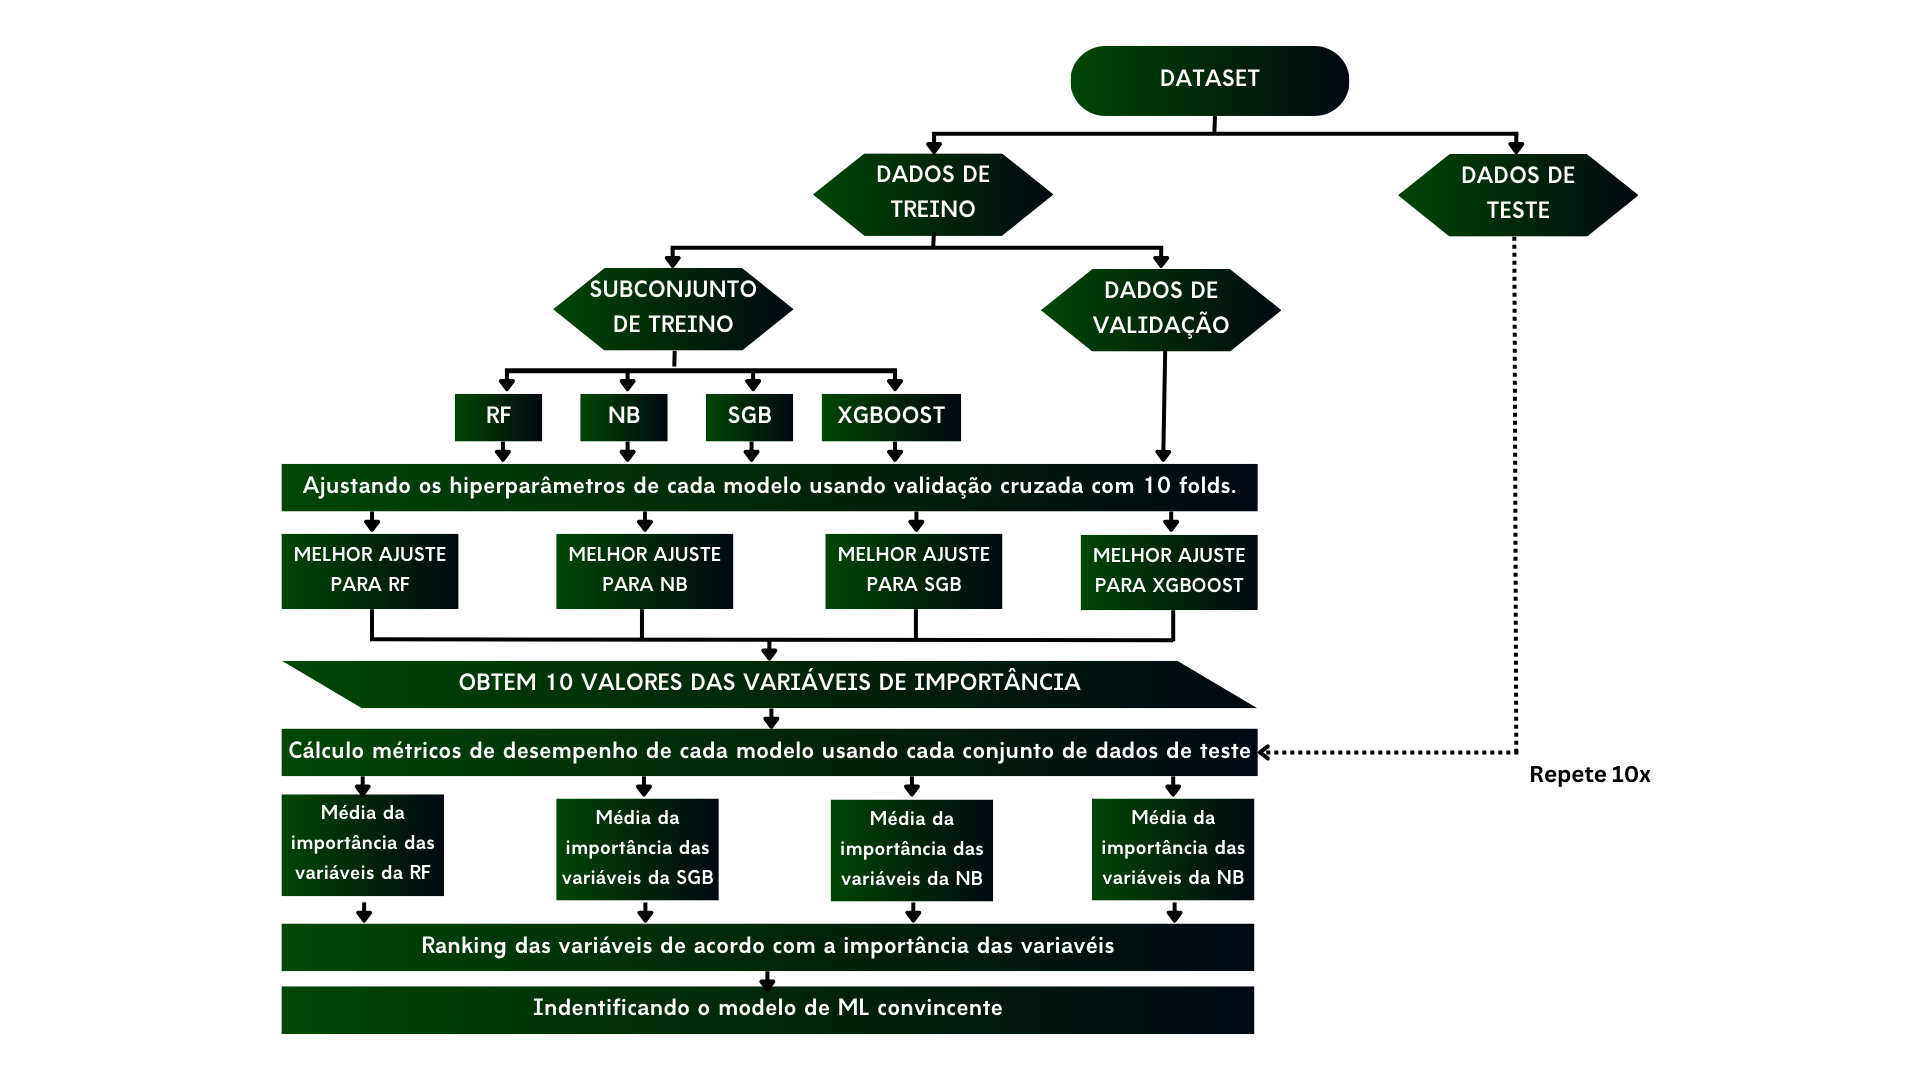
\includegraphics[width=1.2\linewidth, height = !]{imagens//secao3/mlesquema.png}
	\end{figure}
\end{frame}

\begin{frame}{Métricas de Desempenho}
	\centering
	\resizebox{\linewidth}{!}{\begin{tabular}{|>{\centering\arraybackslash}m{4cm}|>{\centering\arraybackslash}m{8cm}|}
		\hline
		\textbf{Métrica} & \textbf{Equação} \\
		\hline
		Erro percentual médio simétrico absoluto & $\displaystyle \text{SMAPE} = \frac{1}{n} \sum_{t=1}^n \frac{|y_t - \hat{y}_t|}{(|y_t| + |\hat{y}_t|)/2} \times 100$ \\
		\hline
		Erro absoluto relativo & $\displaystyle \text{RAIE} = \frac{\sum_{t=1}^n |\hat{y}_t - y_t|}{\sum_{t=1}^n |y_t - \bar{y}|}$ \\
		\hline
		Raiz do Erro Quadrático Relativo & $\displaystyle \text{RRSE} = \sqrt{\frac{\sum_{t=1}^n (\hat{y}_t - y_t)^2}{\sum_{t=1}^n (y_t - \bar{y})^2}}$ \\
		\hline
		Raiz do Erro Quadrático Médio & $\displaystyle \text{RMSE} = \sqrt{\frac{1}{n} \sum_{t=1}^n (\hat{y}_t - y_t)^2}$ \\
		\hline
	\end{tabular}}
\end{frame}

\begin{frame}{Comparação dos métodos}
	\centering
	\begin{tabular}{|c|c|c|c|c|}
		\hline
		\textbf{Modelo} & \textbf{SMAPE} & \textbf{RAE} & \textbf{RRSE} & \textbf{RMSE} \\
		\hline
		LR & 1,3601 & 1,0617 & 1,0459 & 0,6107 \\
		\hline
		RF & 1,3246 & \textbf{1,0185} & 1,0242 & 0,5980 \\
		\hline
		SGB & \textbf{1,2764} & 1,0193 & \textbf{1,0209} & \textbf{0,5961} \\
		\hline
		XGBoost & 1,3601 & 1,0616 & 1,0459 & 0,6107 \\
		\hline
		NB & 1,3385 & 1,0330 & 1,0281 & 0,6003 \\
		\hline
	\end{tabular}
\end{frame}

\begin{frame}{Resultados do Estudo}
	\begin{itemize}
		\item O estudo demonstrou que todos os quatro métodos Mach-L superaram a regressão linear múltipla (MLR) tradicional.
		\item Desempenho dos métodos Mach-L:
		\begin{itemize}
			\item DBP (Pressão Diastólica)
			\item SBP (Pressão Sistólica)
			\item UA (Ácido Úrico)
			\item Nível de escolaridade
			\item TG (Triglicerídeos)
			\item Horas de sono
		\end{itemize}
		\item Identificação dos fatores de risco mais importantes.
	\end{itemize}
\end{frame}

\begin{frame}{}
	\begin{block}{Terço da Misericórdia}
		\aspas{Pela sua dolorosa paixão, tende misericórdia de nós e do mundo inteiro [...] }\textit{(50x)}
	\end{block}
\end{frame}

